\documentclass{utmreport}

\usepackage{booktabs,amssymb,float,graphicx}

\hypersetup{hidelinks,hypertexnames=false,pdfauthor={Lucian-Adrian Gavril}}

\selectlanguage{english}

\utmlogo{utm-logo.jpeg}

\institution{Technical University of Moldova}
\faculty{Faculty of Computers, Informatics, and Microelectronics}
\department{Department of Software Engineering}
\studyprogramme{Software Engineering Study Programme}
\documenttype{Laboratory report}
\reporttitle{Operating Systems Laboratory 4}
\reportsubtitle{The xv6 Shell from the Outside}
\student{Lucian-Adrian Gavril}{FAF-241}
\supervisor{Reițman Patricia}{univ. assist.}
\cityyear{Chișinău}{2026}

\begin{document}
\makeutmreporttitlepage
\tableofcontents
\clearpage

\begin{utmabstract}[Abstract]
This report examines how the xv6 shell turns command text into process execution. It explains file redirection, pipelines, command sequencing, the shell command tree in \texttt{user/sh.c}, and why the built-in \texttt{cd} must run in the parent process. It also inspects the \texttt{sleep} and \texttt{args} utilities and compares their argument handling with GNU Bash. A 9 October 2026 QEMU run verified the no-argument \texttt{sleep} message and \texttt{sleep 20}, which returned to the prompt in 1.96 seconds. A 10 October QEMU run verified all four requested \texttt{args} cases. The screenshots are genuine terminal captures from Dev1 Debian GNU/Linux 13; they do not establish that a course-assigned laptop or VM was used.

\utmkeywords{operating systems, xv6, shell architecture, command line, process hierarchy, argument passing, riscv}
\end{utmabstract}

\utmintroduction
Operating system shells mediate the boundary between user input and kernel process services. A shell parses commands, configures file descriptors, starts processes, creates pipelines, and invokes \texttt{exec()} \cite{cox,love}.

Laboratory 4 examines the xv6 shell (\texttt{user/sh.c}) alongside GNU Bash to identify core shell primitives and the user-space features omitted by xv6. The host did not have a globally installed RISC-V toolchain or QEMU, and \texttt{sudo -n true} returned exit code 1 with \texttt{sudo: a password is required}. Official Debian packages were therefore extracted under a temporary \texttt{/tmp} prefix without installing host packages. On 9 October, \texttt{make qemu} booted a temporary copy of the course tree. A second focused \texttt{make qemu} run on 10 October tested all four argument patterns. The figures below show genuine Bash and QEMU captures from the Dev1 Debian GNU/Linux 13 host; they do not establish that the course-assigned laptop or VM was used.

The investigation is divided into four parts:
\begin{utmenumerate}
\item \textbf{System Call Verification and Sleep Implementation}: Validating the kernel system call declaration in \texttt{user/user.h}, confirming proper argument parsing and tick delays in \texttt{user/sleep.c}, and registering the utility in the xv6 build system.
\item \textbf{Comparative Behavioral Analysis}: Testing identical syntax patterns in Bash and xv6 across I/O redirection, pipelines, list grouping, sequential execution, background jobs, globbing, environment variables, quotation semantics, path searching, and command-line editing.
\item \textbf{Argument Vector Inspection}: Authoring dual implementations of an argument printer (\texttt{args.c} for xv6 and \texttt{args\_linux.c} for Linux) to determine who expands wildcards and strips quotation marks.
\item \textbf{Source Code Architecture of \texttt{user/sh.c}}: Examining the tagged command structures, recursive execution in \texttt{runcmd()}, and the explicit parent-process handling of the \texttt{cd} command.
\end{utmenumerate}

\chapter{System Call Verification and Sleep Implementation}

\section{System call declaration in user.h}
In xv6, system calls available to user programs are prototyped in \texttt{user/user.h}. Because system calls represent kernel traps triggered by assembly stubs in \texttt{usys.S}, the function signatures in \texttt{user.h} must match the dispatch tables in \texttt{kernel/syscall.c}.

The source capture shows the system-call declaration in the copied header (Figure \ref{fig:l4_grep_user_h}) \cite{cox}.

\begin{figure}[H]
\centering
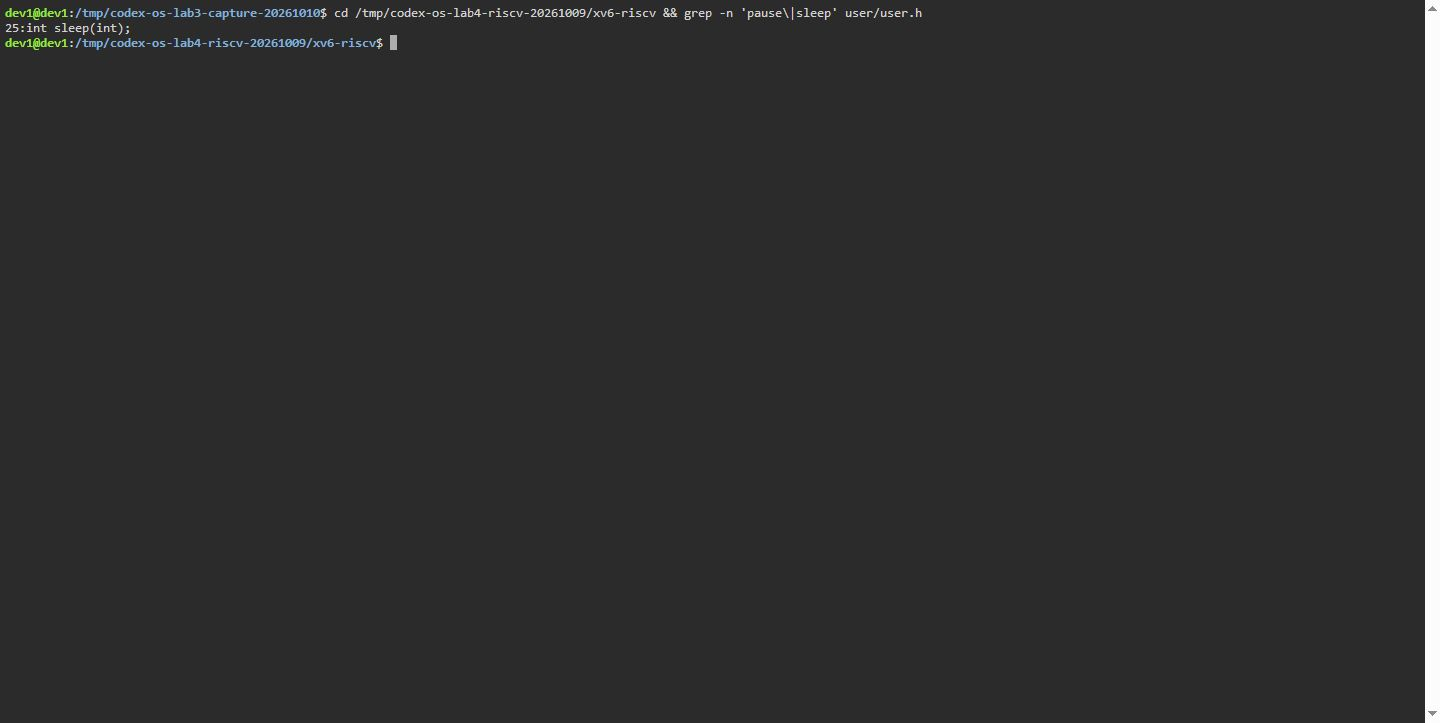
\includegraphics[width=0.88\textwidth]{figures/fig1_1_grep_user_h.jpg}
\caption{Terminal capture, Dev1 Debian GNU/Linux 13, 10 October 2026: System call declaration verified within user/user.h.}
\label{fig:l4_grep_user_h}
\end{figure}

\section{Implementation of user/sleep.c}
The \texttt{sleep} utility serves as an interface between command-line arguments and the kernel timer tick scheduler. The utility verifies that exactly one argument is supplied (\texttt{argc == 2}). If the parameter count is invalid, an error line is emitted to file descriptor 2 (stderr), and the process exits with status 1. If valid, \texttt{atoi()} parses the argument string into an integer and passes it to the system call (Figure \ref{fig:l4_updated_sleep}).

\begin{figure}[H]
\centering
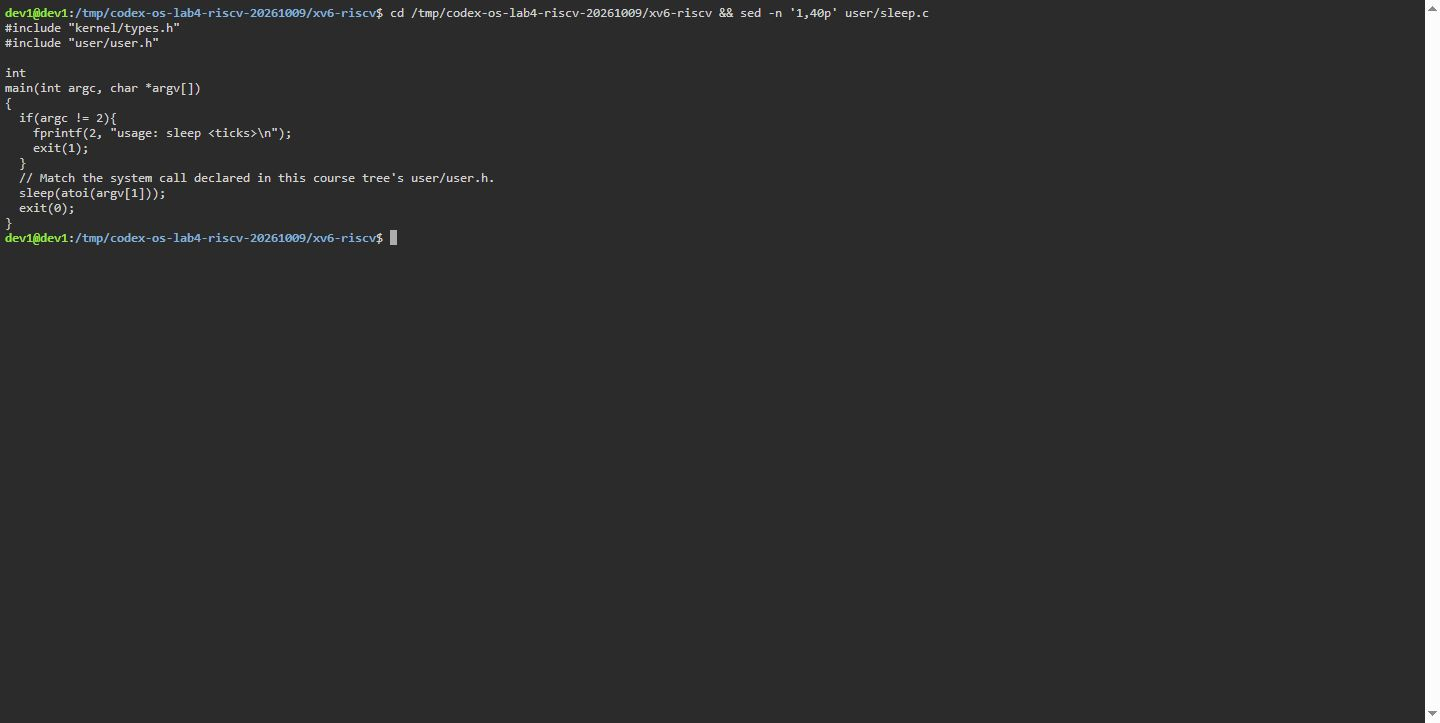
\includegraphics[width=0.88\textwidth]{figures/fig1_2_updated_sleep_c.jpg}
\caption{Terminal capture, Dev1 Debian GNU/Linux 13, 10 October 2026: Implementation of user/sleep.c with input validation.}
\label{fig:l4_updated_sleep}
\end{figure}

\section{Runtime execution in xv6}
The 9 October QEMU run returned to the prompt after \texttt{sleep 20} in 1.96 seconds of measured wall time. It also printed the no-argument usage message and checked two \texttt{args} cases. The following excerpt preserves that earlier serial transcript; the 10 October four-case run is shown in Figure \ref{fig:l4_args_xv6}:

\begin{minipage}{\textwidth}
\small
\begin{verbatim}
init: starting sh
$ sleep
usage: sleep <ticks>
$ sleep 20
$ args one two three
argc = 4
argv[0] = [args]
argv[1] = [one]
argv[2] = [two]
argv[3] = [three]
$ args *.c "x y"
argc = 4
argv[0] = [args]
argv[1] = [*.c]
argv[2] = ["x]
argv[3] = [y"]
$ echo LAB4_SLEEP_DONE
LAB4_SLEEP_DONE
$
\end{verbatim}
\end{minipage}

\begin{figure}[H]
\centering
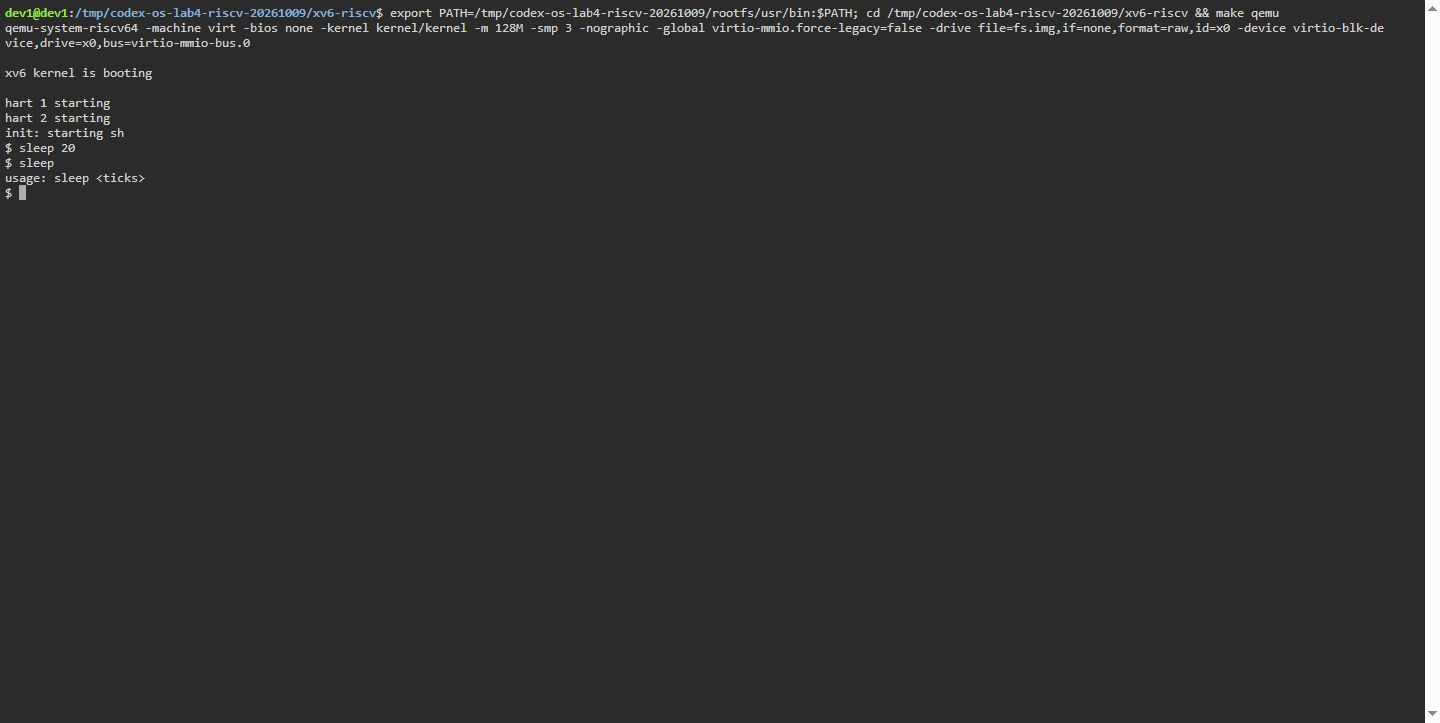
\includegraphics[width=0.88\textwidth]{figures/fig1_3_sleep_run.jpg}
\caption{Terminal capture, Dev1 Debian GNU/Linux 13, 10 October 2026: xv6 boot, \texttt{sleep 20}, and the no-argument usage message.}
\label{fig:l4_sleep_run}
\end{figure}

\chapter{Comparative Architecture: Bash versus xv6 Shell}

\section{Systematic comparison matrix}
The matrix records observed output for nine shell commands and separate keyboard-behavior checks. The Bash and xv6 terminal captures show command rows 1–9; Bash history, completion, and reverse-search behavior and the xv6 line-editing behavior were checked separately. Explanations are based on the course tree and shell source \cite{cox,bach,love}.

\begin{table}[H]
\centering
\small
\setlength{\tabcolsep}{4pt}\begin{tabular}{p{2.6cm}p{3.0cm}p{3.0cm}p{4.6cm}}
\toprule
\textbf{Test Paradigm} & \textbf{Bash Output} & \textbf{xv6 Output} & \textbf{Architectural Explanation} \\
\midrule
\textbf{Redirection} \newline \texttt{echo hello > f ; cat < f} & \texttt{hello} & \texttt{hello} & Both implement \texttt{open()} and \texttt{dup()} redirection via file descriptors. \\
\textbf{Pipe} \newline \texttt{ls | grep READ} & \texttt{README} & \texttt{README} & Both create kernel pipe buffers and coordinate reader/writer via \texttt{pipe()}. \\
\textbf{Grouping} \newline \texttt{(echo a; echo b) | wc} & \texttt{2 2 4} & \texttt{2 2 4} & Both shells accept the tested grouped command in a pipeline; \texttt{wc} reports lines, words, and bytes. \\
\textbf{Sequence} \newline \texttt{echo one ; echo two} & \texttt{one} \newline \texttt{two} & \texttt{one} \newline \texttt{two} & Both implement sequential command execution via \texttt{LIST} nodes separated by \texttt{;}. \\
\textbf{Background} \newline \texttt{echo bg \&} & \texttt{bg} (background) & \texttt{bg} & Both support asynchronous child execution by omitting \texttt{wait()}. \\
\textbf{Globbing} \newline \texttt{ls *} & Lists all entries & \texttt{ls: cannot open *} & Bash performs pathname expansion; xv6 passes literal wildcard characters. \\
\textbf{Variables} \newline \texttt{echo \$HOME} & \texttt{/home/dev1} & \texttt{\$HOME} & Bash expands the host variable; xv6 prints the token literally. \\
\textbf{Quotes} \newline \texttt{echo "a b"} & \texttt{a b} (single arg) & \texttt{"a b"} (literal) & Bash removes quotes and protects whitespace; xv6 splits strictly on spaces. \\
\textbf{PATH Lookup} \newline \texttt{mkdir d ; cd d ; ls ..} & Lists parent-directory entries & \texttt{exec cd failed}; root entries listed & Bash runs \texttt{cd} in the list and uses \texttt{\$PATH}; xv6 tries \texttt{exec cd}, then runs \texttt{ls ..} from \texttt{/}. \\
\textbf{Line Editing} \newline \texttt{Arrows, Tab, \^{}R} & Up: history; Tab: completion; Ctrl+R: reverse search & Up/Ctrl+R: no history or search; blank-prompt Tab: no completion list & Bash behavior was checked interactively. The focused QEMU check found no Up-arrow recall or Ctrl+R search. Blank-prompt Tab produced no completion list; path-prefix completion was not tested. Source inspection shows no such handler in the xv6 console. \\
\bottomrule
\end{tabular}
\caption{Command results for rows 1–9; line-editing behavior was checked separately in Bash and QEMU.}
\label{tab:shell_comparison}
\end{table}

\section{Shell command captures}
The Bash capture shows the nine shell commands run on Dev1 Debian GNU/Linux 13. Up-arrow, Tab, and Ctrl+R behavior was checked separately in an interactive Bash session.

\begin{figure}[H]
\centering
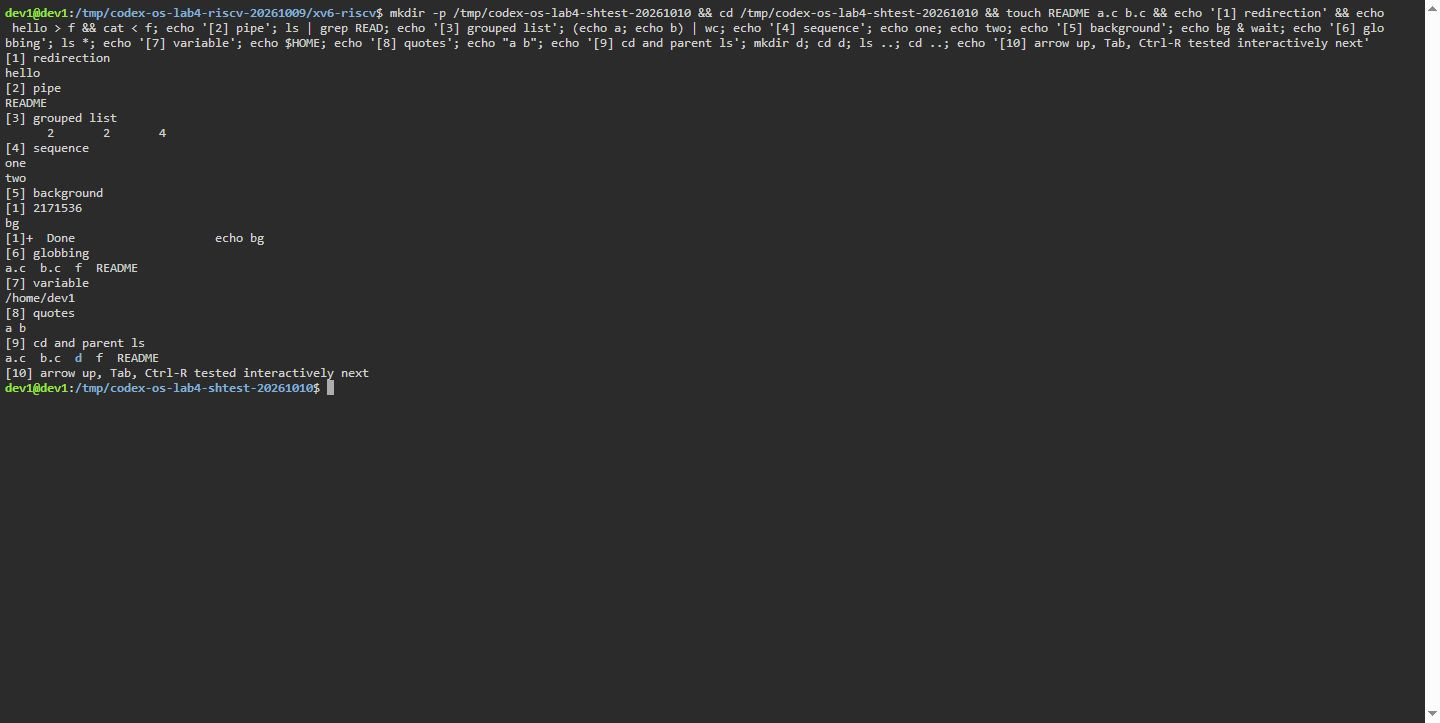
\includegraphics[width=0.88\textwidth]{figures/fig2_1_bash_commands.jpg}
\caption{Terminal capture, Dev1 Debian GNU/Linux 13, 10 October 2026: Bash results for command rows 1 through 9.}
\label{fig:l4_bash_commands}
\end{figure}

The xv6 capture shows nine shell commands. An interaction tested Up, Tab, and Ctrl+R in QEMU: Up and Ctrl+R showed no history or search; Tab at an empty prompt produced no completion list. The console source in \texttt{kernel/console.c}, lines 140–177, handles Ctrl+P, Ctrl+U, Ctrl+H, and Delete. Path-prefix completion was not tested.

\begin{figure}[H]
\centering
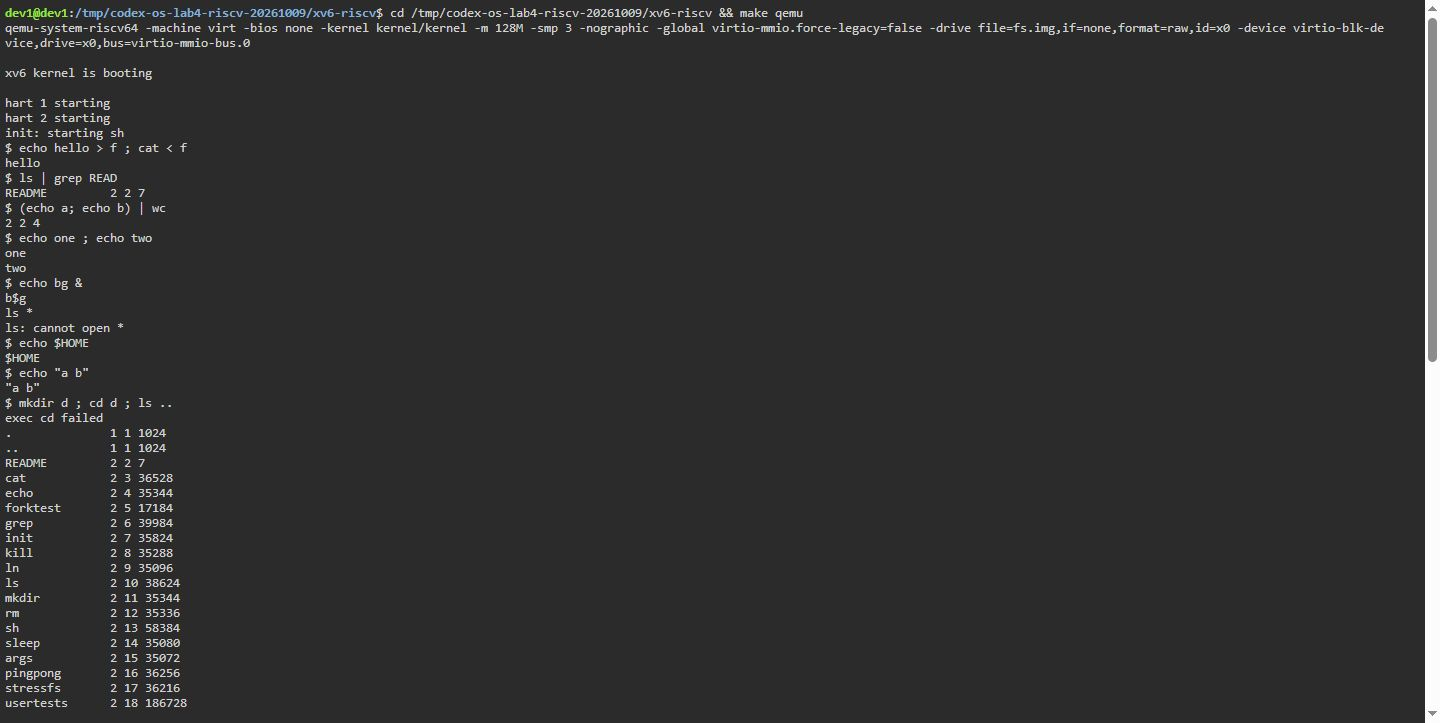
\includegraphics[width=0.88\textwidth]{figures/fig2_2_xv6_commands.jpg}
\caption{Terminal capture, Dev1 Debian GNU/Linux 13, 10 October 2026: xv6 QEMU results for comparison rows 1 through 9.}
\label{fig:l4_xv6_commands}
\end{figure}

\section{Path resolution and directory navigation}
The QEMU capture shows that \texttt{cd d} succeeds at a prompt, a later unqualified \texttt{ls} fails with \texttt{exec ls failed}, and a relative executable path works (Figure \ref{fig:l4_cd_ls_failure}).

\begin{figure}[H]
\centering
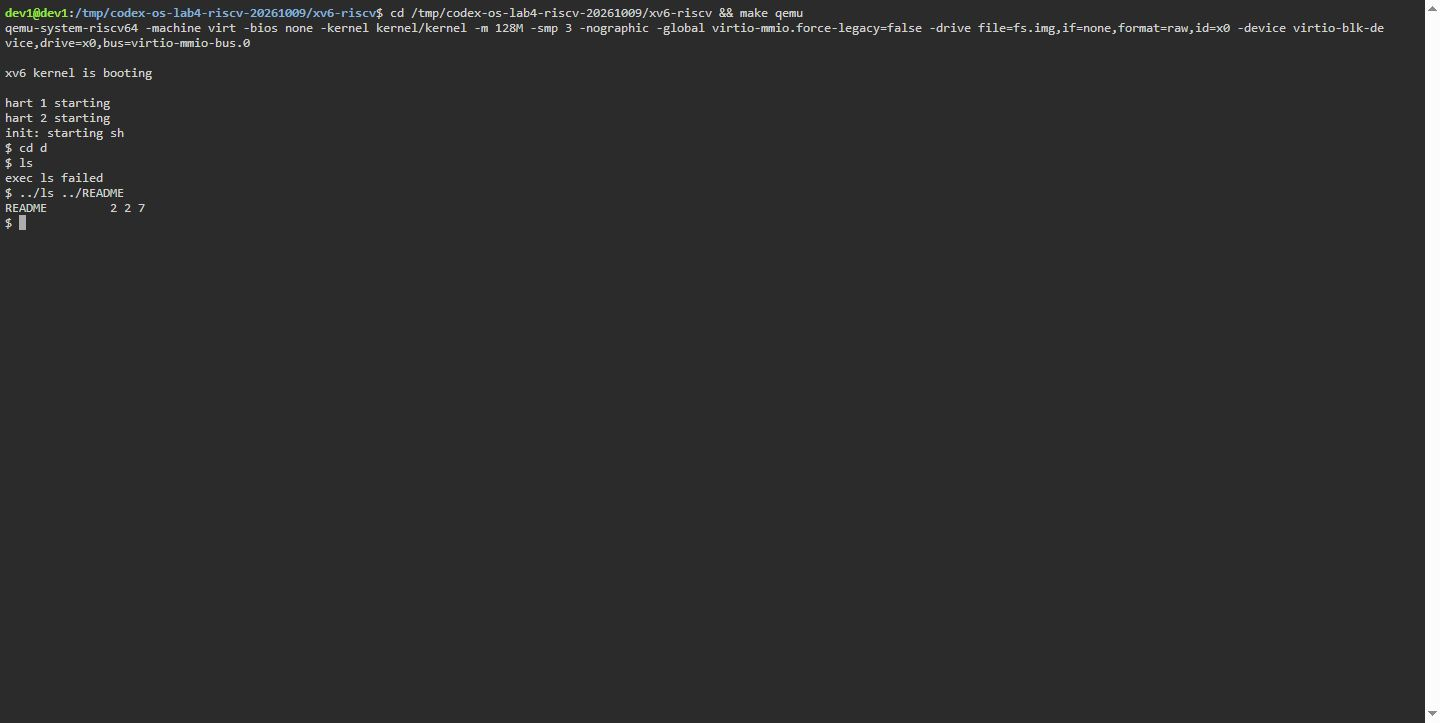
\includegraphics[width=0.88\textwidth]{figures/fig2_3_cd_ls_failure.jpg}
\caption{Terminal capture, Dev1 Debian GNU/Linux 13, 10 October 2026: path lookup after changing directories in xv6.}
\label{fig:l4_cd_ls_failure}
\end{figure}

\section{Answers to Part 2 Observe questions}
\begin{utmenumerate}
\item \textbf{List the features both shells have, and the ones only Bash has.} \\
\textbf{Features in both}: Direct command execution, file descriptor redirection (\texttt{<}, \texttt{>}), pipelines (\texttt{|}), parenthesized command grouping, sequential execution (\texttt{;}), and asynchronous background execution (\texttt{\&}). The grouped xv6 command in the test returned \texttt{2 2 4}. \\
\textbf{Features only in Bash}: Globbing (\texttt{*}, \texttt{?}, \texttt{[...]}), environment variables (\texttt{\$VAR}), quote processing (\texttt{"..."}, \texttt{'...'}), conditional operators (\texttt{\&\&}, \texttt{||}), automatic \texttt{PATH} search, history search, and tab completion.
\item \textbf{In xv6, \texttt{ls} stops working after \texttt{cd d}. Why? Find a way to run \texttt{ls} from inside \texttt{d} anyway.} \\
At the top-level prompt, \texttt{cd d} succeeds. The xv6 shell has no \texttt{PATH} lookup, so \texttt{ls} is resolved relative to \texttt{d} and fails. Figure~\ref{fig:l4_cd_ls_failure} shows the working relative path \texttt{../ls ../README}, which explicitly invokes the executable in the parent directory.
\item \textbf{Which missing feature would you miss most in daily work, and which would be easiest to add?} \\
\textbf{Most missed}: \texttt{PATH} directory resolution and tab completion/history. Without \texttt{PATH}, changing directories renders all core utilities inaccessible unless typed with full paths. \\
\textbf{Easiest to add}: A fallback path search in \texttt{user/sh.c}. If \texttt{exec(cmd, argv)} returns failure, prepend \texttt{"/"} or \texttt{"/bin/"} to \texttt{cmd} and re-execute before returning an error to the user.
\end{utmenumerate}

\chapter{Argument Tokenization: Who Expands Wildcards?}

\section{Implementation of argument vector inspectors}
To demonstrate precisely when and where argument expansions occur, identical inspection utilities were authored for xv6 (\texttt{user/args.c}) and Linux (\texttt{args\_linux.c}). Each prints \texttt{argc} and prints each \texttt{argv[i]} string enclosed in brackets.

\begin{figure}[H]
\centering
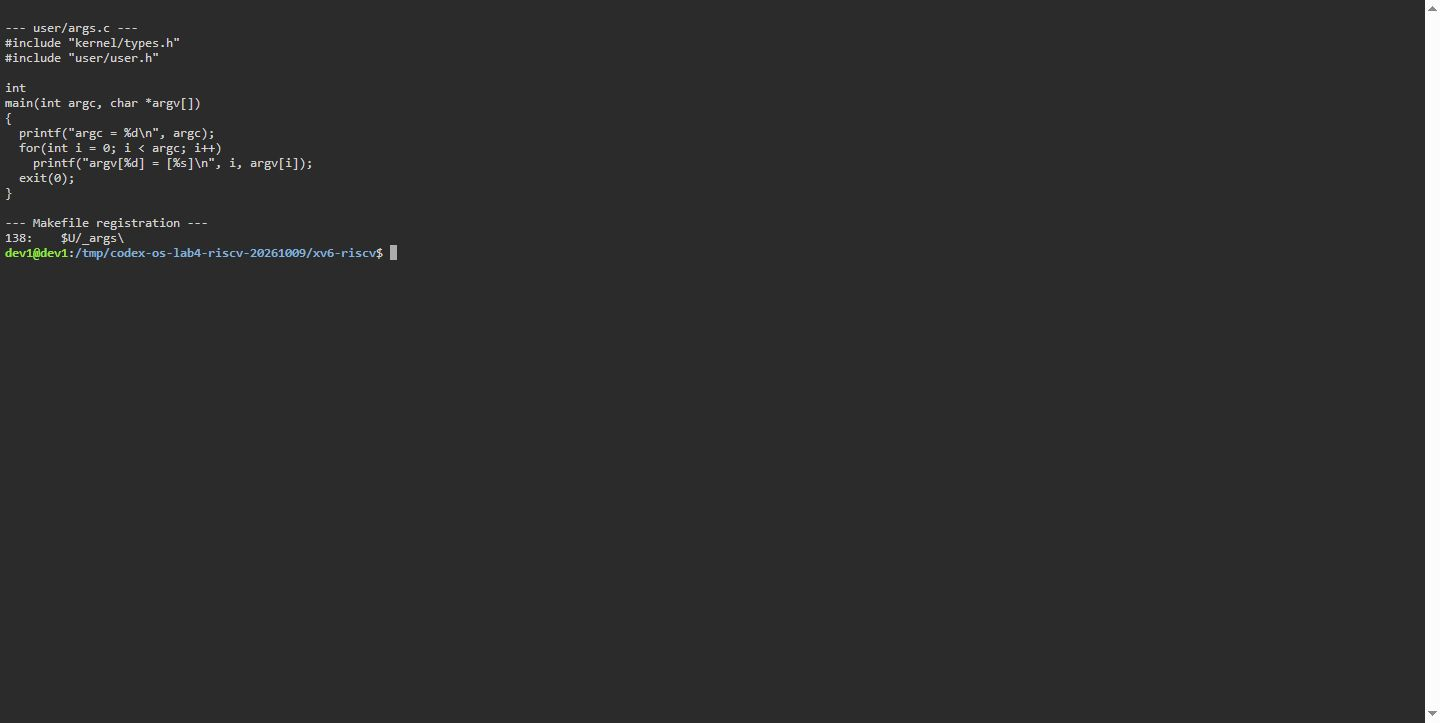
\includegraphics[width=0.88\textwidth]{figures/fig3_1_args_uprogs.jpg}
\caption{Terminal capture, Dev1 Debian GNU/Linux 13, 10 October 2026: Source of user/args.c and registration within xv6 Makefile UPROGS.}
\label{fig:l4_args_uprogs}
\end{figure}

The copied \texttt{Makefile} registers both \texttt{\$U/\_sleep} and \texttt{\$U/\_args} in \texttt{UPROGS}, so the build includes the utilities in \texttt{fs.img}. The capture shows the source and registration lines; the 9 and 10 October QEMU runs built and booted this temporary tree.

\section{Experimental comparison across shells}
Both implementations were run with all four requested argument patterns. The Linux capture used a working directory containing \texttt{a.c}, \texttt{b.c}, and \texttt{args\_linux.c}; the xv6 capture shows the arguments received in QEMU:
\begin{enumerate}
\item \texttt{args one   two   three}
\item \texttt{args *.c "x y"}
\item \texttt{args \$HOME}
\item \texttt{args 'single quoted'}
\end{enumerate}

Figure \ref{fig:l4_args_xv6} shows the actual output from all four xv6 invocations.

\begin{figure}[H]
\centering
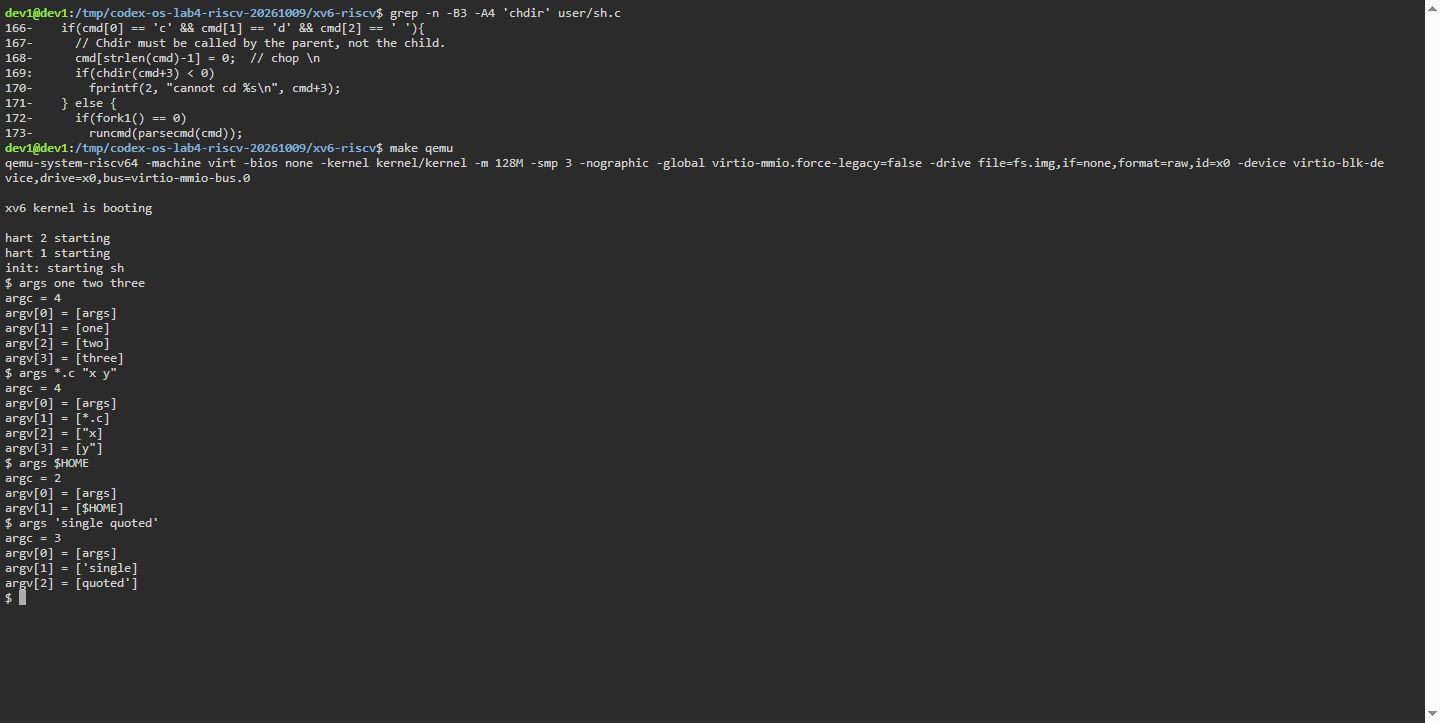
\includegraphics[width=0.88\textwidth]{figures/fig3_2_args_xv6.jpg}
\caption{Terminal capture, Dev1 Debian GNU/Linux 13, 10 October 2026: xv6 output for all four \texttt{args} patterns.}
\label{fig:l4_args_xv6}
\end{figure}

Figure \ref{fig:l4_args_linux} shows the actual Linux Bash output from the same four invocations.

\begin{figure}[H]
\centering
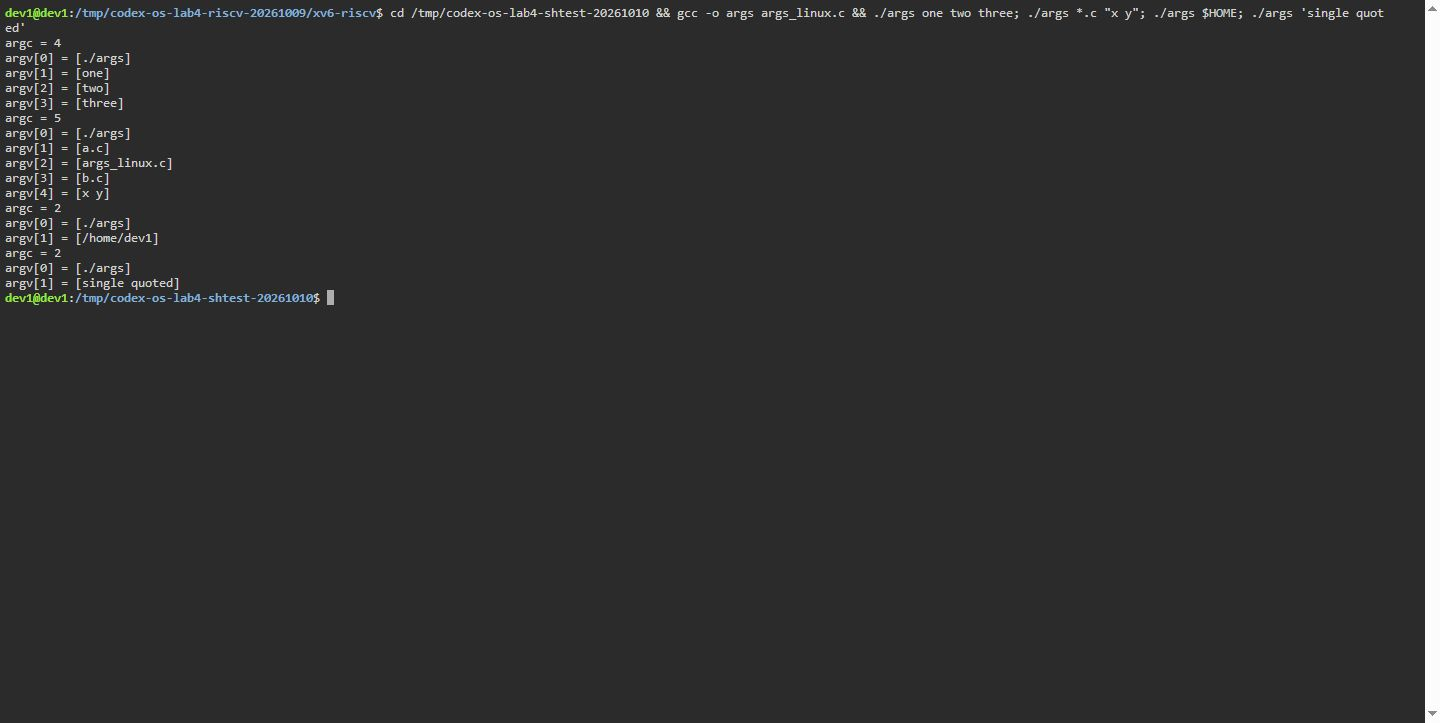
\includegraphics[width=0.88\textwidth]{figures/fig3_3_args_linux.jpg}
\caption{Terminal capture, Dev1 Debian GNU/Linux 13, 10 October 2026: Linux Bash output for all four \texttt{args} patterns.}
\label{fig:l4_args_linux}
\end{figure}

\section{Answers to Part 3 Observe questions}
\begin{utmenumerate}
\item \textbf{Paste both outputs for \texttt{args *.c "x y"}. How many arguments did each program receive?} \\
\textbf{In Linux Bash}:
\begin{verbatim}
argc = 5
argv[0] = [./args]
argv[1] = [a.c]
argv[2] = [args_linux.c]
argv[3] = [b.c]
argv[4] = [x y]
\end{verbatim}
\textbf{In xv6 Shell}:
\begin{verbatim}
argc = 4
argv[0] = [args]
argv[1] = [*.c]
argv[2] = ["x]
argv[3] = [y"]
\end{verbatim}
The Linux program received 5 arguments because the wildcard matched three source files and the quoted phrase remained one argument. xv6 received 4 arguments: it preserved \texttt{*.c} literally and split \texttt{"x y"} into two strings with quotes intact.
\item \textbf{Who turns \texttt{*.c} into file names and removes quotes: the program, the kernel, or the shell?} \\
\textbf{The shell}. The shell performs lexical scanning, globbing, variable expansion, and quote stripping before invoking \texttt{exec()}. The kernel merely accepts an array of already-expanded null-terminated strings and copies them to the new process stack. The user program receives the strings exactly as prepared by the shell.
\item \textbf{What happened to the extra spaces in \texttt{one   two   three}?} \\
The shell treats spaces as argument separators (delimiters). Multiple contiguous spaces are consumed by the lexer during tokenization, so only the non-whitespace tokens (\texttt{"one"}, \texttt{"two"}, \texttt{"three"}) are inserted into the argument array.
\end{utmenumerate}

\chapter{Architecture of user/sh.c}

\section{Command representations and syntax nodes}
The xv6 shell represents commands using tagged C structures. Five command types are defined on lines 8--12 of \texttt{user/sh.c} (Figure \ref{fig:l4_cmd_kinds}):
\begin{itemize}
\item \texttt{EXEC (1)}: Basic command execution; no operator.
\item \texttt{REDIR (2)}: Redirection of I/O; produced by \texttt{<} and \texttt{>}.
\item \texttt{PIPE (3)}: Inter-process communication; produced by \texttt{|}.
\item \texttt{LIST (4)}: Sequential commands; produced by \texttt{;}.
\item \texttt{BACK (5)}: Asynchronous background execution; produced by \texttt{\&}.
\end{itemize}

\begin{figure}[H]
\centering
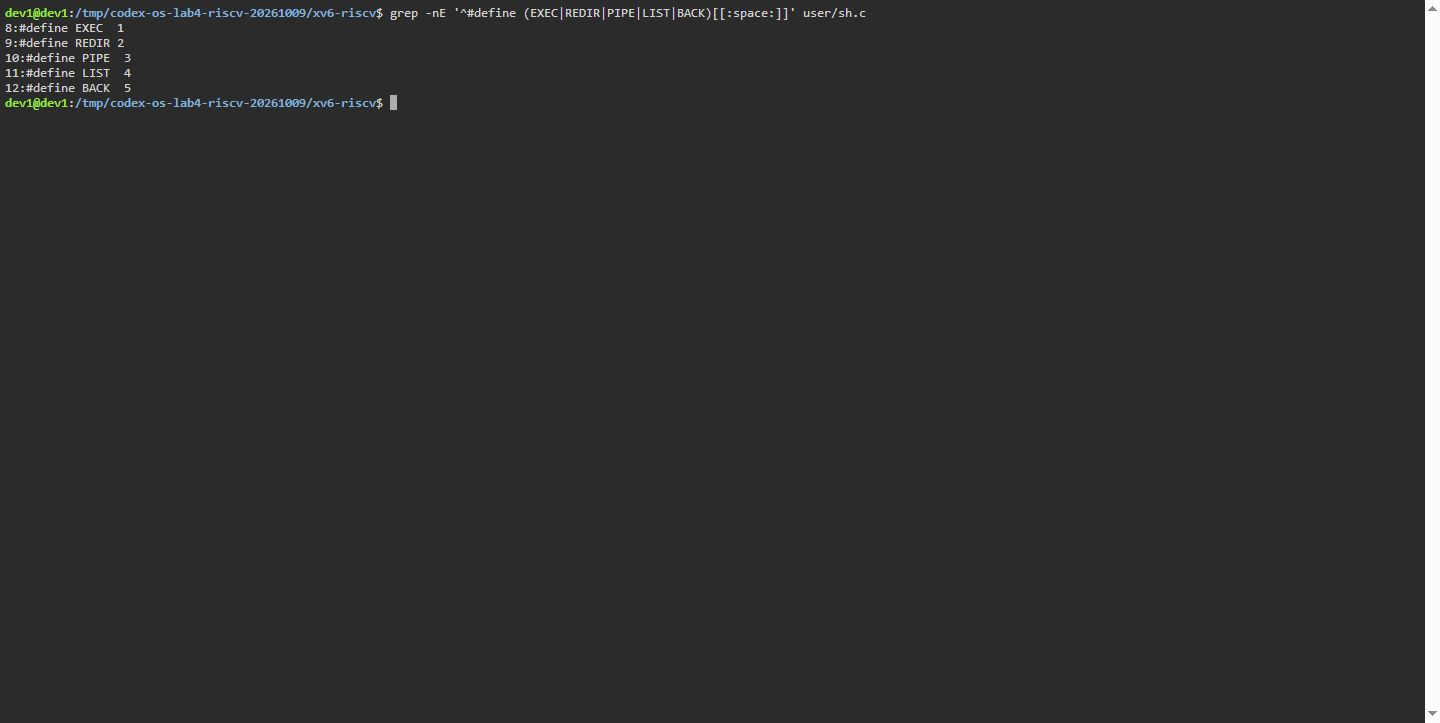
\includegraphics[width=0.88\textwidth]{figures/fig4_1_cmd_kinds.jpg}
\caption{Terminal capture, Dev1 Debian GNU/Linux 13, 10 October 2026: Command types defined in user/sh.c.}
\label{fig:l4_cmd_kinds}
\end{figure}

\section{Recursive command execution in runcmd()}
When a command line is parsed, \texttt{parsecmd()} constructs an abstract syntax tree composed of these structures. The child process then invokes \texttt{runcmd()} \cite{cox} (Figure \ref{fig:l4_runcmd_switch}).

\begin{figure}[H]
\centering
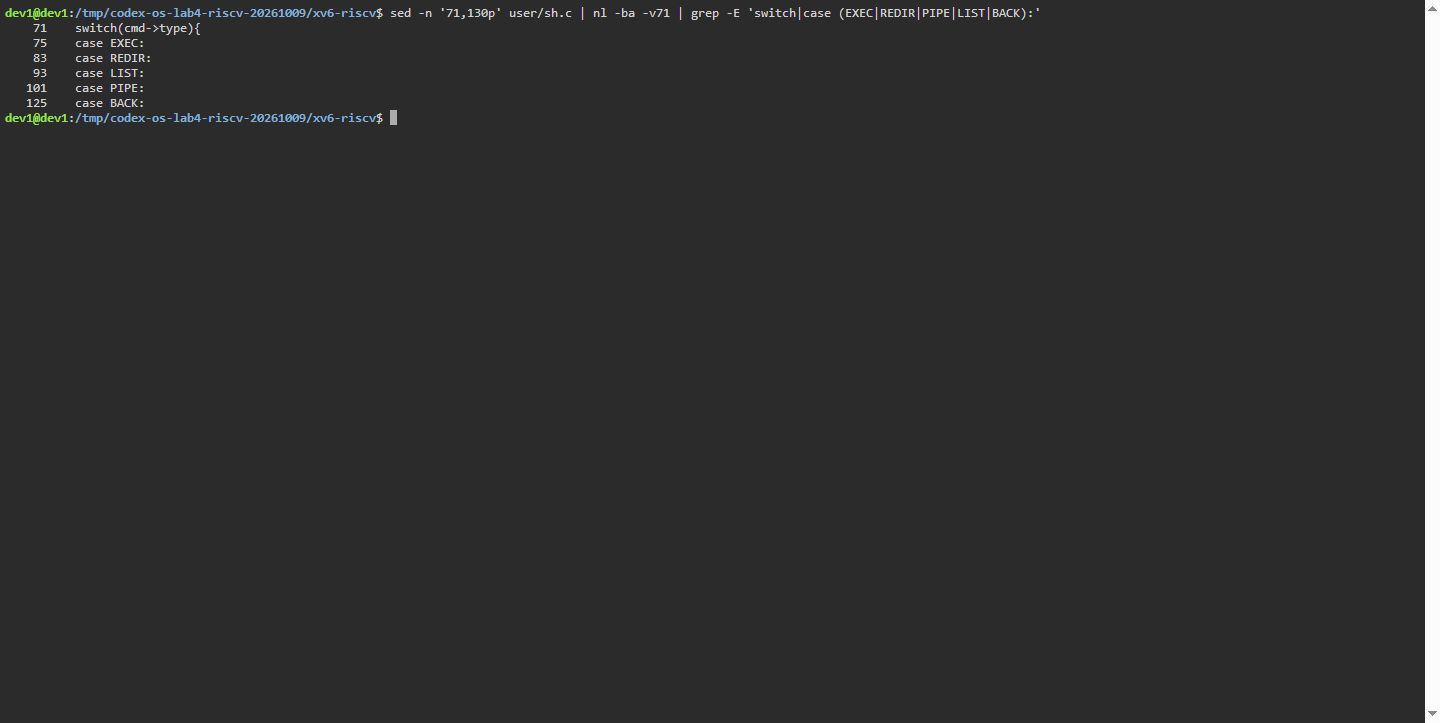
\includegraphics[width=0.88\textwidth]{figures/fig4_2_runcmd_switch.jpg}
\caption{Terminal capture, Dev1 Debian GNU/Linux 13, 10 October 2026: Dispatch switch inside runcmd() handling syntax tree execution.}
\label{fig:l4_runcmd_switch}
\end{figure}

The execution logic handles each node type:
\begin{itemize}
\item For \texttt{EXEC}, it invokes \texttt{exec(ecmd->argv[0], ecmd->argv)}.
\item For \texttt{REDIR}, it closes the targeted descriptor, opens the named file with the requested flags, and recursively evaluates the inner command.
\item For \texttt{PIPE}, it calls \texttt{pipe()}, forks two sub-processes, rewires descriptors 0 and 1 using \texttt{dup()}, closes pipe ends, and waits for both children to terminate.
\item For \texttt{LIST}, it forks a child to run the left command, waits for it, and then runs the right command.
\item For \texttt{BACK}, it forks a child to run the command and immediately returns without waiting.
\end{itemize}

\section{Built-in cd handling and process boundaries}
Lines 166--170 of \texttt{user/sh.c} reveal that \texttt{cd} is explicitly intercepted in the main shell loop before any call to \texttt{fork()} (Figure \ref{fig:l4_cd_handling}).

\begin{figure}[H]
\centering
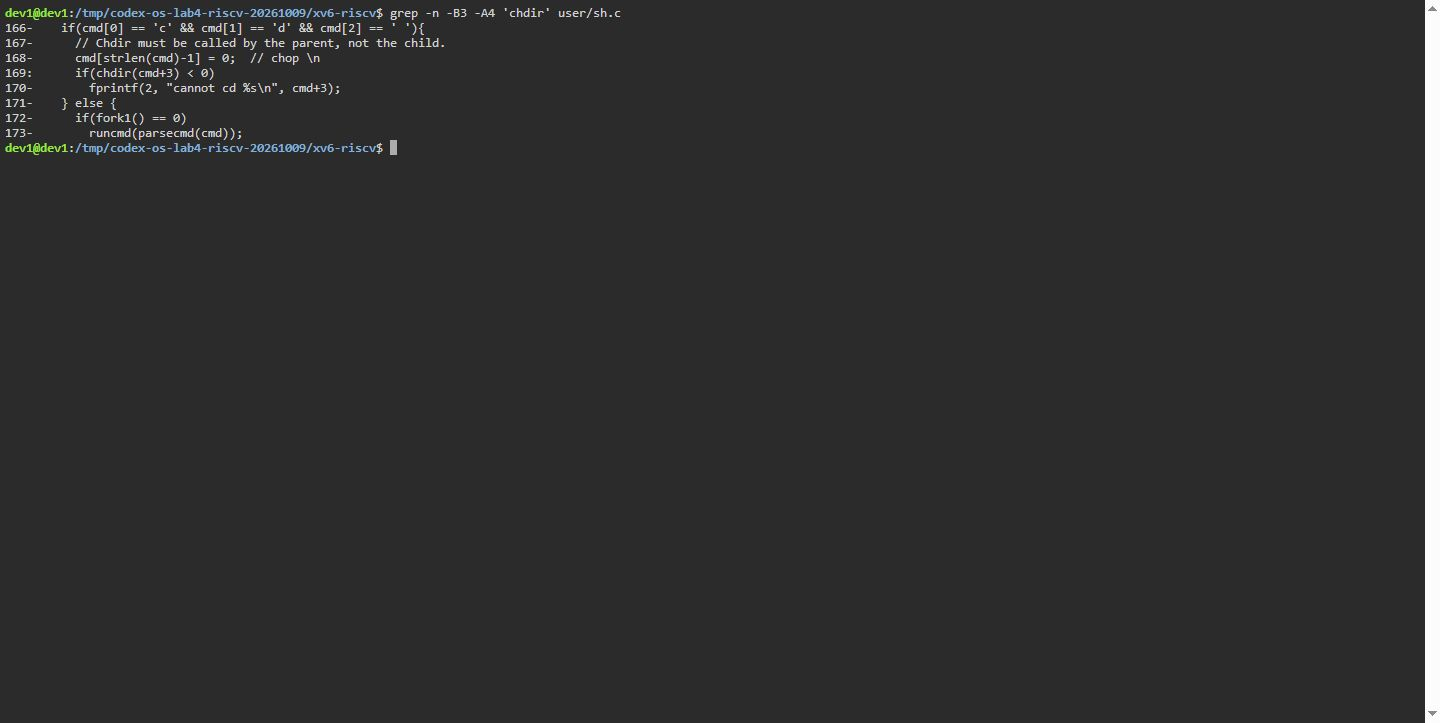
\includegraphics[width=0.88\textwidth]{figures/fig4_3_cd_handling.jpg}
\caption{Terminal capture, Dev1 Debian GNU/Linux 13, 10 October 2026: Parent-process handling of cd built-in in user/sh.c.}
\label{fig:l4_cd_handling}
\end{figure}

\section{Answers to Part 4 Observe questions}
\begin{utmenumerate}
\item \textbf{Name the five kinds of command the xv6 shell knows and the character that produces each.} \\
\texttt{EXEC} (basic command, no special character), \texttt{REDIR} (produced by \texttt{<} and \texttt{>}), \texttt{PIPE} (produced by \texttt{|}), \texttt{LIST} (produced by \texttt{;}), and \texttt{BACK} (produced by \texttt{\&}).
\item \textbf{Where is \texttt{cd} handled, and why is it not run as a separate program?} \\
\texttt{cd} is handled in \texttt{main()} of \texttt{user/sh.c} prior to the \texttt{fork()} call. It cannot be run as a separate program because each child process operates in its own isolated address space and process descriptor table. If \texttt{cd} were an external program, only the child process would change its directory; upon child exit, the parent shell would remain in the original directory. Therefore, \texttt{chdir()} must execute directly in the parent shell process.
\item \textbf{Search \texttt{sh.c} for any code that handles \texttt{*} or \texttt{\$}. What does that explain about Part 2?} \\
Searching \texttt{sh.c} reveals zero code handling \texttt{*} or \texttt{\$}. Neither globbing nor variable expansion logic exists in the parser. This explains why \texttt{echo \$HOME} and \texttt{ls *} print literal characters in xv6: the shell treats them as ordinary alphanumeric tokens and passes them uninspected to \texttt{exec()}.
\end{utmenumerate}

\utmconclusions
The captures distinguish Bash expansion from xv6 token splitting, while the source figures identify the xv6 command types and parent-process handling of \texttt{cd}. A focused QEMU check found no Up-arrow recall or Ctrl+R search, and Tab at an empty prompt produced no completion list. Source inspection confirms that the xv6 console has no history, completion, or reverse-search handler; path-prefix completion was not tested.

\begin{thebibliography}{9}
\bibitem{cox} Cox, R., Kaashoek, M. F., \& Morris, R. (2023). \textit{xv6: a simple, Unix-like teaching operating system}. MIT CSAIL.
\bibitem{patterson} Patterson, D. A., \& Hennessy, J. L. (2017). \textit{Computer Organization and Design RISC-V Edition}. Morgan Kaufmann.
\bibitem{love} Love, R. (2013). \textit{Linux System Programming: Talking Directly to the Kernel and C Library} (2nd ed.). O'Reilly Media.
\bibitem{bach} Bach, M. J. (1986). \textit{The Design of the UNIX Operating System}. Prentice-Hall.
\end{thebibliography}

\end{document}
